\newpage 
\section{Failure Models}

\label{sec:failures}
\subsection{Defining Failures}
This section discusses, what to do or how to classify when failures occur.

\begin{Def}[Failure Model]

    A \textbf{Failure Model} is a set of assumptions about the types of failures that can occur in a distributed system.
    Such failures may be \textbf{Correlated} or \textbf{Independent}. Processes that do not fail are considered \textbf{Correct}.
\end{Def}

\noindent
In particular, we are concerned with the following types of failures:
\begin{itemize}
    \item Crash and or omission of responses, and how we might recover from them.
    \item Deviation protocol, arbitrarily or maliciously.
\end{itemize}
\begin{Def}[Crash-Stop Failure]
    
    \label{def:crash-stop}
    A \textbf{Crash-Stop Failure} occurs when a process halts and does not resume (e.g., power failure, software crash). The failure is not explicitly detectable by other processes.
    \textbf{Permanent hardware failures} typically fall under category of crash-stop failures.\\
\end{Def}

\noindent

\begin{Def}[Fail-Stop Failure]
    
    A \textbf{Fail-Stop Failure} is a detectable crash-stop failure (e.g., timeouts, heartbeats).
\end{Def}


\begin{Def}[Omission Failure]

    An \textbf{Omission Failure} can be categorized into two types:

    \begin{itemize}
        \item \textbf{Send Omission}: The process fails to send messages according to the protocol.
        \item \textbf{Receive Omission}: The process fails to receive messages that were sent by other processes.
    \end{itemize}

    \noindent
    \textbf{In particular}, The process itself may still be operational but unable to correctly communicate (e.g., network disruptions, software errors, or buffer overflows).
\end{Def}

\newpage 

\begin{Def}[Crash-Recovery Failure]

    A \textbf{Crash-Recovery Failure} occurs when a process halts due to a crash but retains the \textbf{ability to recover} and resume execution. 

    \begin{itemize}
        \item \textbf{Crash Phase}: The process halts in some way (e.g., stops sending or receiving messages).
        \item \textbf{Recovery Phase}: The processes may recover to the last correct state via snapshot (\ref{sec:snap}). Certain types of memory may persist through the crash:
        \begin{itemize}
            \item \textbf{Volatile memory} is lost during a crash (e.g, mid-execution variables).
            \item \textbf{Stable storage} is retained through a crash (e.g., disk storage, assuming no disk failure).
        \end{itemize}
    \end{itemize}

    \noindent
    \textbf{However,} if the processes crashes indefinitely, it is considered a \textbf{Crash-Stop} failure (\ref{def:crash-stop}).
\end{Def}

\begin{Def}[Byzantine Failure]

    A \textbf{Byzantine Failure} occurs when a process exhibits arbitrary or malicious behavior, leading to unpredictable system behavior.

    \begin{itemize}
        \item \textbf{Arbitrary Behavior}: The process deviates from the expected protocol, such as:
        \begin{itemize}
            \item Sending corrupted or inconsistent messages to different nodes.
            \item Updating its state in an unintended or unpredictable manner.
        \end{itemize}

        \item \textbf{Malicious Behavior}: The process actively attempts to disrupt the system, such as:
        \begin{itemize}
            \item Exploiting protocol vulnerabilities to manipulate outcomes (e.g., double-spending in a blockchain).
        \end{itemize}
    \end{itemize}

    \noindent
    In short, these failures occur due to \textbf{bugs} (unintentional) or \textbf{attacks} (intentional).
\end{Def}

\begin{Tip} The term \textbf{Byzantine} in computer science comes from the \textit{Byzantine Generals Problem}, introduced by Leslie Lamport in 1982. It describes a scenario where generals must coordinate an attack but cannot trust all messengers—some may be traitors sending conflicting information.

    The name \textit{Byzantine} is inspired by the Byzantine Empire, which was historically known for its complex and often deceptive political intrigues. While the term is widely used in distributed systems, some argue it unfairly portrays Byzantine history.

    In computing, a \textbf{Byzantine failure} refers to a system component acting unpredictably, whether due to bugs, faults, or malicious intent, making consensus difficult.

\end{Tip}

\newpage

\subsection{Failures Model Hierarchy}

Here we compare failure models as extensions of each other, though we will omit \textbf{fail-stop} as it is more of a detection mechanism.
To quickly recap:
\begin{itemize}
    \item \textbf{Crash-Stop}: Process halts and cannot resume (undetectable).
    \item \textbf{Omission}: Process fails to properly communicate.
    \item \textbf{Crash-Recovery}: Process halts but can recover and resume.
    \item \textbf{Byzantine}: Process exhibits arbitrary or malicious behavior.
\end{itemize}

\begin{theo}[Failure Model Hierarchy]

    The failure models can be arranged in a hierarchy, where each model is an extension of the previous one. 
    The hierarchy is as follows:
    \begin{center}
        \textbf{Crash-Stop} $\subset$ \textbf{Omission} $\subset$ \textbf{Crash-Recovery} $\subset$ \textbf{Byzantine}
    \end{center}
    In particular, 
    \begin{itemize}
        \item \textbf{Crash-Stop} $\subset$ \textbf{Omission}: A crash-stop is a full crash rather than a partial communication failure.
        \item \textbf{Omission} $\subset$ \textbf{Crash-Recovery}: During recovering the last correct state, volatile memory lost may exhibit omission-like behavior. Meaning some messages are lost due to ``\textbf{amnesia}.''
        \item \textbf{Crash-Recovery} $\subset$ \textbf{Byzantine}: as a process may recover and exhibit arbitrary or malicious behavior. Moreover, a Byzantine failure may be \textbf{any type of failure}.
    \end{itemize}
\end{theo}

\begin{figure}[h]
    \centering
    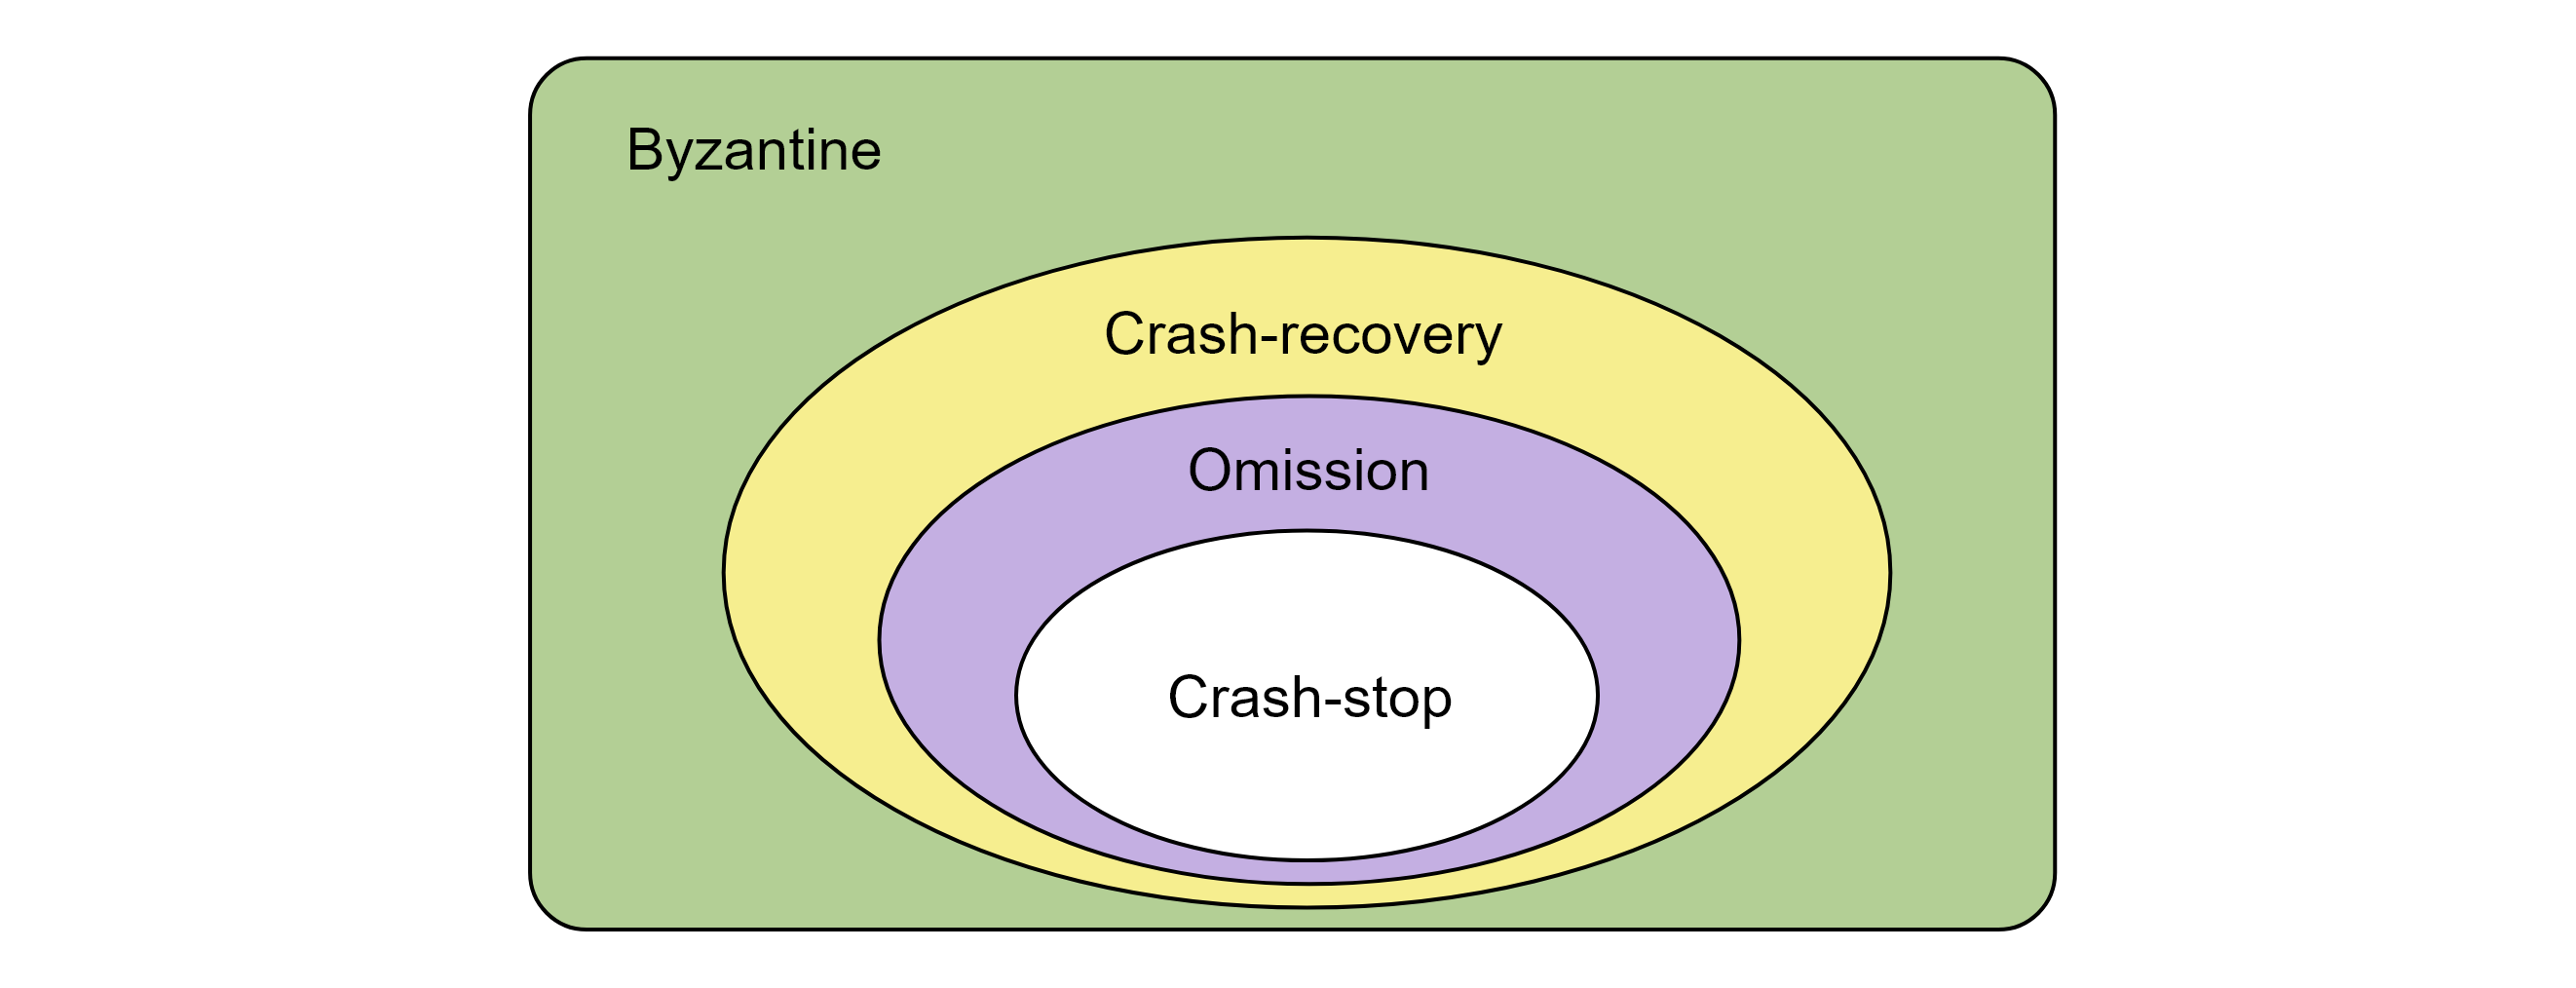
\includegraphics[width=\textwidth]{Sections/crash/fail.png}
    \caption{Failure Hierarchy depicting: Crash-stop $\subset$ Omission $\subset$ Crash-Recovery $\subset$ Byzantine}
\end{figure}



